\chapter{Introduction}

\label{chapter:introduction}

In this chapter, we introduce this thesis by presenting its motivation,
describing our research questions and providing an overview of the thesis
structure. We start off by considering the current trend of utilizing
increasingly large deep learning models to address Machine Learning (ML)
and Natural Language Processing (NLP) tasks.

\section{Motivation}

With the recent trend of increasingly large deep learning models achieving
State-Of-The-Art (SOTA) performance on a myriad of ML tasks
including in NLP as shown in Figure \ref{fig:nlp_progress}, several studies argue for
focused research into Explainable Artificial Intelligence (XAI) to address
emerging concerns such as security risks and inductive biases associated with
black-box models
\citep{doran2017does,townsend2019extracting,danilevsky2020survey,arrieta2020explainable}.

Of these studies, \citet{arrieta2020explainable} provide an extensive overview
of XAI and related concepts based on a thorough literature review of $\sim$400
XAI research contributions published to date. In particular,
\citet{arrieta2020explainable} explore and classify a variety of
machine-learning models into transparent and black-box categories depending on
their degrees of transparency. Furthermore, they explore taxonomies of post-hoc
explainability techniques aimed at effectively explaining black-box models. Of high
relevance to this thesis are the local explanations, feature relevance and
explanations by simplification post-hoc explainability techniques.

Through our own survey of recent literature on explainability techniques used
in NLP, we came across several interesting studies employing the local
explanations, feature relevance and explanations by simplification
explainability techniques to better explain black-box models; particularly
deep neural networks.
\citep{schwartz2018sopa,peng2018rational,suresh-etal-2019-distilling,wang2019state,jiang2020cold}.
Drawing inspiration from the work of \citet{schwartz2018sopa}, we focus this
thesis on further developing their \textbf{So}ft \textbf{Pa}tterns (SoPa) model;
which represents a hybridized RNN, CNN and Weighted Finite-State Automaton (WFA)
neural network architecture. We modify the SoPa model by changing key aspects of
its architecture which ultimately allows us to conduct effective explanations by
simplification and abbreviate this modified model as \textbf{SoPa++}, which
signifies an improvement or major modification over the SoPa model. Finally, we
evaluate both the performance and explanations by simplification of the SoPa++
model on the Facebook Multilingual Task Oriented Dialog data set (FMTOD;
\citealt{schuster-etal-2019-cross-lingual}); focusing on the English-language
intent classification task.

\begin{figure}[th]
  \centering
  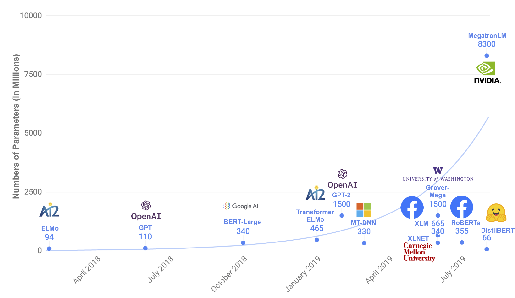
\includegraphics[width=13cm]{pdfs/borrowed/nlp_sota_model_size_progress.pdf}
  \caption{Parameter counts of recently released pre-trained language models
    which showed competitive or SOTA performance when fine-tuned over a range of
    NLP tasks; figure taken from \citet{sanh2019distilbert}}
  \label{fig:nlp_progress}
\end{figure}

\section{Research questions}

With the introduction of our SoPa++ model, we aim to answer the following three
research questions:

\begin{enumerate}
  \item To what extent does SoPa++ contribute to competitive
  performance\footnote{We define competitive performance as the scenario where a
    mean performance metric on a certain task falls within the range
    obtained from other recent studies on the same task} on the FMTOD
  English language intent classification task?
  \item To what extent does SoPa++ contribute to effective explanations by
  simplification on the FMTOD English language intent classification task?
  \item What interesting and relevant explanations can SoPa++ provide on the
  FMTOD English language intent classification task?
\end{enumerate}

\section{Thesis structure}

With the aforementioned research questions, we summarize the structure and
contents of this thesis.

\begin{description}[align=left]
  \item [Chapter \ref{chapter:introduction}:] Introduce this thesis, its
  contents and our research questions.
  \item [Chapter \ref{chapter:background}:] Describe the background concepts
  utilized in this thesis.
  \item [Chapter \ref{chapter:methodologies}:] Describe the FMTOD data set and
  methodologies pursued in this thesis.
  \item [Chapter \ref{chapter:results}:] Describe the results obtained from our
  methodologies.
  \item [Chapter \ref{chapter:discussion}:] Interpret and discuss the
  implications of the aforementioned results.
  \item [Chapter \ref{chapter:conclusions}:] Conclude this thesis by answering
  the research questions.
  \item [Chapter \ref{chapter:further_work}:] Document future work to expand on
  our research questions.
\end{description}

%%% Local Variables: 
%%% mode: latex
%%% TeX-master: "main"
%%% End: 

% LocalWords:  SOTA XAI explainability NLP Automata FAs WFAs FMTOD th nlp pre
% LocalWords:  sota tterns
